\newpage
\section{Paralelní běh programů}
Python rozlišuje dva typy paralelismu: vícevláknový (multithreading) a víceprocesový (multiprocessing) běh. Vlákna poskytují pouze iluzi skutečného paralelismu: pro jeden proces Pythonu (tj. jedno spuštění \verb|python file.py|) běží v jednom okamžiku pouze jedno vlákno, ale běh se přepíná mezi více vlákny tak, aby se vytvořila iluze paralelismu. I když váš skript běží na vícejádrovém (nebo víceprocesorovém) počítači, bude použito pouze jedno jádro\footnote{Od verze Pythonu 3.13 lze \emph{globální zámek interpretu, global interpreter lock} (GIL), který způsobuje, že vlákna běží bez skutečného paralelismu, volitelně vypnout, ačkoli GIL zůstane výchozím chováním v dohledné budoucnosti. Více podrobností viz \href{https://docs.python.org/3.13/whatsnew/3.13.html\#whatsnew313-free-threaded-cpython}{zde}.}. Víceprocesový paralelismus na druhé straně může spouštět více procesů Pythonu skutečně paralelně, současně na více jádrech CPU, pokud jsou k dispozici.

Ačkoli se vlákna mohou zdát zbytečná, často se snadněji používají a zejména pro aplikace, které čekají na hardwarové I/O, síť nebo interakci s uživatelem, jsou často lepší volbou. Víceprocesové aplikace mohou být rychlejší pro dostatečně velké problémy, avšak pro krátce běžící programy jsou často \emph{pomalejší}, protože správa více procesů vyžaduje \emph{režii}, která může být srovnatelná s řešením samotného problému.

\subsection{Vícevláknový paralelismus (Multithreading)}

\ls{Thread} objekty z modulu \ls{threading} reprezentují vlákna. Vlákna provádějí danou \emph{cílovou} (target) funkci, když jsou \emph{spuštěna}, a po dokončení musí být \emph{připojena} (joined) zpět k rodičovskému vláknu. Příklad použití:
\lstinputlisting{../example_code/threads_baisc.py}

Často je však objektově orientovaný přístup pohodlnější než target funkce. Můžeme definovat vlastní objekty vláken jednoduchým děděním z \ls{Thread} a definováním metody \ls{run()}. Funkčně ekvivalentní příklad k výše uvedenému:
\lstinputlisting{../example_code/threads_oop.py}

Vlákna musí být schopna vzájemně komunikovat a předvídatelně sdílet zdroje. Zvažte VISA funkci \ls{query()}, což je jednoduše \ls{write()} okamžitě následované \ls{read()}. Pokud existují dvě vlákna komunikující se stejným zařízením Pico, jedno provádí \ls{query(':READ:P?')} a druhé \ls{query(':READ:T?')}, existuje šance, že skutečné pořadí provedených čtení a zápisů bude:

\begin{tabular}{cc}
\begin{lstlisting}[linewidth=0.49\linewidth]
    # vlákno 1
    write(':READ:P?')
    # běží vlákno 2
    # běží vlákno 2
    read()
\end{lstlisting}&
\begin{lstlisting}[linewidth=0.49\linewidth]
    # vlákno 2
    # běží vlákno 1
    write(':READ:T?') 
    read()
    # běží vlákno 1
\end{lstlisting}
\end{tabular}\\
a vlákno, které žádalo o tlak, dostane teplotu a naopak. Tato třída chyb se nazývá \emph{souběh} (race conditions) -- tj. dvě vlákna se „předhánějí“ v soutěži o zdroj a vítěz je náhodný. Abychom tomu zabránili, musíme Pythonu říci, že bychom neměli být na chvíli přerušeni, dokud neskončíme se zápisem a čtením. Toho se dosahuje pomocí \emph{zámků} (nebo mutexů, z MUTual EXclusion), které jsou k dispozici v modulu \ls{threading} jako třída \ls{Lock} a používají se následovně\\
\begin{tabular}{cc}
\begin{lstlisting}
    from threading import Lock
    lock = Lock()
\end{lstlisting}& \\
\begin{lstlisting}[linewidth=0.4\linewidth]
    # vlákno 1
    lock.acquire()
    # běží vlákno 2
    write(':READ:P?')
    read()
    lock.release()
    # běží vlákno 2
    # běží vlákno 2
    # běží vlákno 2
\end{lstlisting}&
\begin{lstlisting}[linewidth=0.6\linewidth]
    # vlákno 2
    # běží vlákno 1
    lock.acquire() # blokuje, dokud není zámek uvolněn
    # běží vlákno 1
    # běží vlákno 1
    # běží vlákno 1, lock.acquire() se vrátí
    write(':READ:T?') 
    read()
    lock.release()
\end{lstlisting}
\end{tabular}

Všimněte si, že používáme objekt vytvořený třídou \ls{Lock}, nikoli třídu samotnou. To platí pro všechny synchronizační a komunikační mechanismy -- \ls{Lock}s, \ls{Event}s a \ls{Queue}s a další. Zámky podporují protokol správy kontextu, takže je obvykle používáme v příkazu \ls{with} místo přímého volání \ls{acquire()} a \ls{release()}. Úplnější příklad,
\lstinputlisting{../example_code/threads_locks.py}

Všimněte si, že pokud bychom použili dva zámky k uzamčení dvou samostatných zdrojů, mohli bychom se dostat do situace, kdy dva zámky na sebe navzájem čekají věčně, jako je tato\\
\begin{tabular}{cc}
\begin{lstlisting}[linewidth=0.5\linewidth]
    # vlákno 1
    # snaží se získat lock1 a lock2
    # v tomto pořadí
    lock1.acquire()
    # běží vlákno 2
    # běží vlákno 2
    lock2.acquire() # blokuje navždy
\end{lstlisting}&
\begin{lstlisting}[linewidth=0.5\linewidth]
    # vlákno 2
    # snaží se získat lock2 a lock1
    # v tomto pořadí
    # běží vlákno 1
    lock2.acquire() 
    lock1.acquire() # blokuje navždy
    # běží vlákno 1
\end{lstlisting}
\end{tabular}\\
což se nazývá \emph{zablokování} (deadlock). Buďte zvláště opatrní, když používáte více než jeden zámek.

Nejjednodušší metodou komunikace mezi vlákny jsou globální proměnné. To se však může rychle stát nepřehledným a matoucím, proto je obvykle lepší používat typy určené pro komunikaci mezi vlákny. Nejjednodušší je \ls{threading.Event}, což je booleovský příznak, který může být nastaven jedním vláknem a na který může reagovat jiné, např.:
\lstinputlisting{../example_code/threads_events.py}

Pro posílání dat mezi vlákny jsou užitečné \ls{Queue}s z modulu \ls{queue}. Hodnotu můžeme vložit do fronty v jednom vlákně pomocí metody \ls{put()} a vyjmout ji jinde pomocí metody \ls{get()}, která blokuje, pokud je fronta prázdná. Můžeme také zkontrolovat, zda je fronta prázdná, pomocí metody \ls{empty()}. Minimální příklad:
\lstinputlisting{../example_code/threads_queues_minimal.py}

Úplnější příklad, který čte data z Pico v jednom vlákně a vykresluje je v jiném:
\lstinputlisting{../example_code/threads_queues.py}

\begin{exercise}
    Napište program, který bude blikat všemi 5 LED diodami separátně v intervalech 0.1, 0.2, 0.5, 1 a 2 s.
\end{exercise}

\begin{exercise}
    Napište program, který bude zobrazovat aktualizovaný graf tlaku. Během běhu programu by měl být schopen přijímat textové příkazy a měl by podporovat: clear, který vymaže aktuální graf, a quit, který program čistě ukončí.
\end{exercise}

\subsection{víceprocesový paralelismus (Multiprocessing)}
Víceprocesový paralelismus může využívat více jader CPU, avšak existují omezení na to, jaké druhy proměnných lze sdílet mezi procesy. Nové procesy můžeme vytvářet pomocí třídy \ls{Process} z modulu \ls{multiprocessing} velmi podobným způsobem jako vlákna. Modul \ls{multiprocessing} také poskytuje synchronizační a komunikační prostředky podobné \ls{threading}, tj. \ls{Event}, \ls{Queue} atd. Musíte však používat třídy z modulu multiprocessing pro komunikaci mezi procesy. Minimální příklad, kde hlavní proces vytváří sadu procesů a posílá jim všem zprávy prostřednictvím sdílené \ls{Queue}:
\lstinputlisting{../example_code/multiprocessing_process.py}

Výše uvedený kód je příkladem \emph{fondu procesů} (process pool), což je často nejjednodušší způsob, jak urychlit problémy, které zahrnují více nezávislých výpočtů. Multiprocessing již poskytuje obecný fond process pool pro tento úkol:
\lstinputlisting{../example_code/process_pools_minimal.py}
který aplikuje funkci \ls{function(x)} na každý prvek sekvence (např. seznam, pole, ...) v 6 paralelních procesech a sbírá výsledky.

Úplnější příklad, který počítá Fibonacciho posloupnost pomalaým rekurzivním algoritmem:
\lstinputlisting{../example_code/process_pools.py}
všimněte si, že pro přílišné zvětšení počtu procesů může výpočet ve skutečnosti začít \emph{spomalovat}.

\subsection{Meziprocesová komunikace}
Doposud jsme vytvářeli nové procesy z python skriptu, který jsme spustili. Avšak jakékoli dva procesy Pythonu, tj. samostatné běhy jakýchkoli programů v Pythonu, mohou spolu komunikovat. Existuje několik způsobů, jak toho dosáhnout, například přímé sdílení paměti (pomocí modulu \ls{multiprocessing.shared_memory}, viz \href{https://docs.python.org/3/library/multiprocessing.shared_memory.html}{dokumentaci} pro příklad použití s poli numpy) nebo \emph{sokety}. Mechanismus soketů je nějakým způsobem poskytován všemi operačními systémy jako obecný způsob komunikace mezi procesy, lokálně nebo přes síť, viz Obr.~\ref{fig:listener-client}. Obecně navážeme spojení s adresou (může být \emph{localhost}, pokud nekomunikujeme přes síť) a číslem portu. Jeden proces funguje jako \emph{posluchač} (tj. server), který \emph{přijímá} spojení od \emph{klientů} a oba si pak mohou navzájem posílat a přijímat zprávy.

\begin{figure}
    \label{fig:listener-client}
    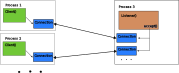
\includegraphics[width=\textwidth]{listener_client.pdf}
    \caption{Vztahy mezi posluchači, klienty a spojeními}
\end{figure}

Níže uvedený příklad ukazuje jednoduchý echo server -- server, který jednoduše posílá zpět klientovi to, co obdrží. Bude přijímat pouze spojení z lokálního počítače na portu 6000. Nejprve je objekt posluchače vytvořen pomocí příkazu \ls{with}, který je poté použit ke spuštění samostatného vlákna, které přijímá spojení a odpovídá klientům. Hlavní vlákno bude jednoduše čekat na signál k ukončení. Pokud máme skončit, zavřeme posluchače (musíme také odblokovat \ls{accept()}, které by čekalo věčně) a skončíme. Všimněte si, že hesla jsou volitelná, pokud nezadáte \ls{authkey} pro \ls{Listener}, nemusíte ho zadávat ani pro \ls{Client}.

Klient je v porovnání mnohem jednodušší. Jednoduše se připojte k posluchači se známou adresou, portem a heslem a můžete začít posílat a přijímat data. Metody \ls{send()} a \ls{recv()} provádějí serializaci a deserializaci (pickling a unpickling, vzpomeňte si na pickling ze souborů \ls{.npy}), takže lze posílat téměř všechny objekty Pythonu.

Pro otestování níže uvedeného příkladu spusťte \verb|python server.py| v jedné konzoli a \verb|python client.py| v druhé.

\ls{server.py}:
\lstinputlisting{../example_code/ipc_server.py}

\ls{client.py}
\lstinputlisting{../example_code/ipc_client.py}

Pro povolení spojení ze sítě jednoduše zadejte adresu posluchače jako \ls{''} (prázdný řetězec) a připojte se s klientem k IP adrese počítače, na kterém běží proces posluchače. Pozor na to, že pickling a unpickling v \ls{send()} a \ls{recv()} může vést k potenciálním bezpečnostním problémům, takže je nejlepší použít heslo, pokud přijímáte spojení přes síť.

\begin{exercise}
Server běží na počítači s IP adresou \verb|<IP>|, na portu \verb|<PORT>| s heslem \verb|<PASSWORD>|. Tento server ovládá Pico přímým odesláním jakéhokoli řetězce, který obdrží, do Pico a odesláním odpovědi z Pico zpět. Připojte se k tomuto serveru s klientem, odešlete příkaz \verb|*IDN?| pro dotaz na identifikaci přístroje a blikněte LED diodou, pokud je odpověď správná.
\end{exercise}

\verb|instrument_server.py|:
Kód přijímá spojení v samostatném vlákně. Pro každé přijaté spojení spustí nové vlákno pro obsluhu klienta. Všechna vlákna pro obsluhu klienta sdílejí stejné Pico, takže ho musíme před pokusem o komunikaci řádně uzamknout, protože nás může kdykoli přerušit jiný klient. Server se ukončí, když obdrží KeyboardInterrupt (Ctrl-C).
\lstinputlisting{../example_code/instrument_server.py} %

\subsubsection{Reálný případ použití v laboratoři}
Na Obr.~\ref{fig:networking-usecase} je fotografie jednoho počítače, který ovládá tři experimenty připojené ke dvěma různým experimentálním sestavám. Každý experiment patří jinému studentovi, který může potřebovat spouštět a upravovat své měřicí skripty v Pythonu současně, takže jednoduché sdílení vzdálené plochy není k dispozici.

Nakonec jsme použili server pro přístroje podobný zjednodušenému příkladu výše, který studentům umožnil spouštět měřicí skripty na jakémkoli počítači ve stejné síti, dokonce i na jejich vlastních noteboocích.

\begin{figure}
    \label{fig:networking-usecase}
    TODO
    \caption{Jeden počítač ovládající více experimentů.}
\end{figure}